\begin{document}

\def\title{CSM Test}

\newcommand{\qitem}{\qpart\item}
\newcommand{\test}{../../testing}

\renewcommand{\labelenumi}{(\alph{enumi})} % change default enum format to (a)
\renewcommand{\theenumi}{(\alph{enumi})} % fix reference format accordingly.
\renewcommand{\labelenumii}{\roman{enumii}.} % second level labels.
\renewcommand{\theenumii}{\roman{enumii}.}

\maketitle

\vspace{0.5em}

\qcontributor{Taejin Hwang}

\section{How to Write Proofs}

This guide was written to provide some useful tips on how to approach and overcome your fear on writing proofs. 
A couple examples of proofs are given, and the details are a bit exaggerated, but they do emphasize the importance of the following tips below. They were mainly exaggerated to show which step of the proof corresponds with which tip.

% \begin{enumerate}[label=(\roman*)]
\subsection{Know your definitions}
This is the single most important piece of advice I can give, a proof will always require you to know your definitions. 
From my experiences with teaching, when a student is stuck on a proof, it is almost always because they didn't remember a definition.

For example, a question asks to prove that a set of vectors is linearly independent, you will need to know what linear independence means, and you may have to know multiple definitions of linear independence to finish the proof. 

\subsection{Identify your Goal}
Often times, proof questions may get really long, and you forget what the goal of the proof was. 
It is always important to identify what you want to prove at the beginning and continually refer back to it while proving. 
Another strategy that you may need to use, is to identify the objective, and then ask yourself, "Can I rephrase this objective into something else that makes the problem easier?" 
This ability to do this will come from a strong understanding of definitions.

For example, if a questions asks you to prove two vectors $\vec{u}, \vec{v}$ are orthogonal, you may want to think about what it means to be orthogonal and maybe rephrase it as: Can I show $\vec{u}^{T} \vec{v} = 0?$

\subsection{Try Something!}
This is perhaps the scariest part of the proof. 
You may \textbf{not} want to try something because you think it will lead to a wrong answer, but only after you try will you actually be able to say so. 
The best way to start a proof is to write out definitions you know that are related to the problem, and then seeing which ones are the most helpful.

For example, if a question asks to prove:
$$|\innp{\vec{u}}{\vec{v}}| \leq \norm{\vec{u}} \norm{\vec{v}},$$ 
then try writing out all the definitions of the inner product you know and you'll see that the cosine definition is most useful here.

\subsection{Intuition}
This is the hardest of them all, and are the reason why even some of the best mathematicians struggle with proofs.
Think of a proof as a puzzle where the pieces are your definitions, but knowing which definitions will be more useful than others, or having the idea to multiply both sides by a term, comes from this magical word. 
This comes from \textbf{practice}, \textbf{reading}, and \textbf{understanding} a large number of proofs.

Some techniques that will come from intuition are multiplying and dividing by a certain constant, adding and subtracting $0,$ or maybe even interpreting the geometry of a problem.

For example.

\subsection{Use all the information given!}
Happens to me all the time. I try writing a proof, I go step by step, but then hit a dead end. 
This is when you should go back, and check, \textbf{is there any assumption or fact given in the statement that I have not used yet?}
As a general tip, if a question gives a "weird" fact or assumption, you will most likely have to use that assumption somewhere in your proof.

\subsection{Organization}
The worst feeling when writing a proof is when something you need is written on your paper, but your work is too messy for you to realize it's sitting right in front of you. 
Make sure you clearly document what your steps were one by one, and to keep track of your definitions one by one so you don't lost anything in the mess of everything.

\section{Example}
Q: Show that a set of non-zero vectors that are mutually orthogonal are linearly independent.
\begin{enumerate}
 \item \textbf{Definitions:} We should recall the definition of orthogonality. 
  Two vectors are orthogonal if their inner product is zero, or $\innp{\vec{u}}{\vec{v}} = 0.$ 
  We should also then think about the definitions of an inner product and how $\innp{\vec{u}}{\vec{v}} = \vec{u}^{T} \vec{v}.$
 \item \textbf{Goal:} The goal is to show that these orthogonal vectors are linearly independent.
 This means that if $\alpha_{1} \vec{v}_{1} + \dotsc + \alpha_{n} \vec{v}_{n} = \vec{0},$ then all of the scalars must be zero.
 We should keep this in mind, while constructing our proof.
 \item \textbf{First Step / Plan:} What should we write on our paper? With our goal in mind, we should probably write out 
 $$\alpha_{1} \vec{v}_{1} + \dotsc + \alpha_{n} \vec{v}_{n} = \vec{0}$$
 and then somehow show all of the $\alpha_{i}$ must be zero.
 \item \textbf{Intuition:} We have now established our goal of showing all of the $\alpha_{i}$ must be zero.
 But we are unsure of how to get there. We should use the fact that these vectors are \textbf{orthogonal} in some way or another. 
 Since two vectors are orthogonal when $\vec{u}^{T} \vec{v} = 0,$ and we know that $\vec{v}_{1}^{T} \vec{v}_{i} = 0$ for $i \neq 1,$ our intuition should tell us that we should multiply both sides by $\vec{v}_{1}^{T}$ and see what happens.
 \item \textbf{Try Something:} Let's try taking the inner product of both sides with $\vec{v}_{1},$ ask yourself why this is equivalent to multiplying both sides by $\vec{v}_{1}^{T}.$ Then we see that
 $$\vec{v}_{1}^{T} (\alpha_{1} \vec{v}_{1} + \dotsc + \alpha_{n} \vec{v}_{n}) = \vec{v}_{1}^{T} \vec{0}$$
 We need to remember our definitions (specifically the distributive property of inner products and vector multiplication).
 We should also remember that the inner product with the $\vec{0}$ will alwyas be zero.
 $$\alpha_{1} \vec{v}_{1}^{T} \vec{v}_{1} + \dotsc + \alpha_{n} \vec{v}_{1}^{T} \vec{v}_{n} = 0$$
 \item \textbf{Organization:}
 There is a lot to keep track of even in a proof as simple as this one. We need to remember why we multiplied by $\vec{v}_{1}^{T}$ to begin with. We did it since all of the $\vec{v}_{i}$ were orthogonal, and as a result, we should now see that all of the terms should be zero, \textbf{except} $\vec{v}_{1}^{T} \vec{v}_{1}!$

 But now you should be asking yourself, "what if $\vec{v}_{1}$ is zero, then $\vec{v}_{1}^{T} \vec{v}_{1}$ would be equal to $0?"$ While this is a concern to have, since if $\vec{v}_{1}^{T} \vec{v}_{1} = 0,$ it would say nothing about $\alpha_{1},$ we must remember our original assumption that \textbf{the vectors were non-zero.} 
 Therefore $\vec{v}_{1}^{T} \vec{v}_{1} = \norm{\vec{v}_{1}}^{2}$ must be greater than zero by the positive-definiteness of norms. 
 Looking back at the original equations, we see that 
 $$\alpha_{1} \vec{v}_{1}^{T} \vec{v}_{1} = 0$$
 so since $\vec{v}_{1}^{T} \vec{v}_{1} > 0,$ we know for sure that $\alpha_{1}$ must be zero.

 \item \textbf{Conclusion:}
 We've tried taking the inner product of both sides with $\vec{v}_{1}$ and shown that $\alpha_{1}$ must be zero and should now be suspecting that all of them are zero, but how can we show that all of the $\alpha$ are zero? 
 We can do this by generalizing the argument saying, "Hey what if I took the inner product of both sides with $\vec{v}_{i}$ for any $i = 1, \dots, n?$" If I can show $\alpha_{i} = 0,$ then it would mean $\alpha_{1}, \dots, \alpha_{n}$ are all equal to zero. In this case, we are allowed to do so, and therefore, conclude by saying all of the $\alpha_{i}$ are zero. 
 Therefore, we conclude the proof by stating, "Since all of the $\alpha_{i} = 0,$ vectors $\vec{v}_{1}, \dots, \vec{v}_{n}$ must be linearly independent."

\end{enumerate}


\section{Example}

Q: Prove that if $A$ is a matrix of full rank, then every eigenvalue of the matrix $A^{T}A$ will be greater than $0.$ \textit{Hint: Consider $\norm{A\vec{v}}^{2}$ where $\vec{v}$ is an eigenvector of $A^{T}A.$}

\begin{enumerate}
 \item \textbf{Definitions:} Before we even start, we should recall the definitions for full rank, eigenvalues, and norms. 
 I'm not going to list the individual definitions here, but remember that you will most likely have to use all of these definitions somewhere in the proof.
 \item \textbf{Goal:} In some way or another, we must show that every eigenvalue $\lambda$ of the matrix $A^{T}A$ must be greater than zero. Algebraically we can express this as showing $\lambda > 0$ for every $\lambda$ of the matrix $A^{T}A.$
 \item \textbf{Using Information / Intuition:} If a question gives a hint, \textbf{use the hint!} To build some intuition behind the hint, we want to look at eigenvalues of $A^{T}A \vec{v} = \lambda \vec{v}$ the norm of $\norm{A\vec{v}}^{2} = (A \vec{v})^{T} (A \vec{v}) = \vec{v}^{T} A^{T} A \vec{v}.$ 
 Without the hint, the intuition would've to construct $A^{T}A \vec{v}$ since we want to show every eigenvalue is greater than or equal to zero, and then focus on how we can show something is greater than zero. 
 The term $A^{T}A \vec{v}$ is very close to $\vec{v}^{T} A^{T} A \vec{v}$ which is equal to $\norm{A \vec{v}}$ and we know that norms are always greater than or equal to zero.
 This should explain the intuition behind the hint, and the thought process that would've been taken without the hint.
 \item \textbf{Try Something!:} Now let's actually take the hint as is and consider this value $\norm{A\vec{v}}^{2}.$ 
 As stated in the previous step, we can expand out the this squared norm to get $\vec{v}^{T} A^{T} A \vec{v}.$
 Since the hint told us to look at the specific vector $\vec{v}$ which is an eigenvector of $A^{T}A,$ we should use this fact to say that $$\norm{A \vec{v}}^{2} = \vec{v}^{T} \lambda \vec{v} = \lambda \vec{v}^{T} \vec{v}.$$
 It may seem like we are stuck now, but we are actually almost there! 
 The key here is to now think back to the goal. 
 Our goal was to show that $\lambda > 0.$ 
 So let's look at the information we currently have. We have $\norm{A \vec{v}}^{2} = \lambda \vec{v}^{T} \vec{v}.$
 Since we want to isolate the $\lambda$ on its own, we should try playing with $\vec{v}^{T} \vec{v},$ and we can make the observation that $\vec{v}^{T} \vec{v} = \norm{\vec{v}}^{2}.$ 
 I would consider this observation under the \textit{intuition} category, and it really comes from the idea of seeing that we need to isolate $\lambda$ and show that it's greater than zero, and the fact that norms are also greater than zero. 
 \item \textbf{Organization:} We're almost there, but we still have cleaning up to do. We now have the expression
 $$\norm{A \vec{v}}^{2} = \lambda \norm{\vec{v}}^{2}$$
 We spent a lot of time discussing why we should be isolating $\lambda$ so you should be thinking of diving by $\norm{\vec{v}}^{2}$but then you should also ask yourself: "How do I know that $\norm{\vec{v}}^{2} \neq 0?$" 
 Dividing by zero would be a disaster and this proof would break down from here.
 However, remember that $\vec{v}$ was defined to be an eigenvector of $A^{T}A$ meaning the vector will be nonzero, and its norm will henceworth be nonzero as well.
 With all of this in mind, we now divide and end up with the expression:
 $$\lambda = \frac{\norm{A\vec{v}}^{2}}{\norm{\vec{v}}^{2}}$$
 We know that $\norm{\vec{v}}^{2} > 0,$ since $\vec{v} \neq \vec{0},$ and $\norm{A\vec{v}}^{2} \geq 0$ since norms are greater than or equal to zero, we can say that $\lambda \geq 0.$ However our goal was to show that $\lambda$ is strictly greater than zero. How could we achieve this? We could achieve this is we could show that $\norm{A\vec{v}}^{2} > 0.$ 
\item \textbf{Use all the information given!:}
 We may feel stuck again at this point, so let's go back to the original problem statement and see if there is any information that we have not used yet. It happens that we haven't used the fact that $A$ is full rank anywhere in the proof yet! 
 It is no conicidence that this is the exact fact that we need to finish up the proof, without it we could only say that each eigenvalue of $A^{T}A$ is greater than or equal to zero. Since $A$ is a matrix of full rank, the matrix equation $A \vec{x} =\vec{0}$ will have the unique solution $\vec{x} = \vec{0}.$ We were looking at norm of $A \vec{v}$ where $\vec{v}$ is nonzero since $\vec{v}$ is an eigenvector of $A^{T}A.$ Using the fact that $A$ is full rank and  $\vec{v} \neq \vec{0},$ we should see that $A \vec{v}$ must also be nonzero. Since we are squaring the norm of a nonzero vector, $\norm{A\vec{v}}^{2} > 0,$ and we can conclude that $\lambda$ must be strictly greater than zero.
\end{enumerate}


% \section{Example}

% Q: Prove t


% \begin{qunlist}

% % Authors: Taejin Hwang
% Emails: taejin@berkeley.edu

\qns{System Identification}

In this question, we will take a look at how to \textbf{identify} a system by taking experimental data taken from a (presumably) linear system to learn a discrete-time linear model for it using the least-squares.

Recall that a \textbf{linear, continuous-time,} system can be put in state-space form:
\begin{equation}
\ddt{}{t} \vec{x}(t) = A \vec{x}(t) + \vec{b} u(t)
\end{equation}

Now let's say we have an \textbf{unknown} linear system in which we can give an input $u(t)$ and observe the output $\vec{x}(t).$ We can model the system using the following diagram:
\begin{center}
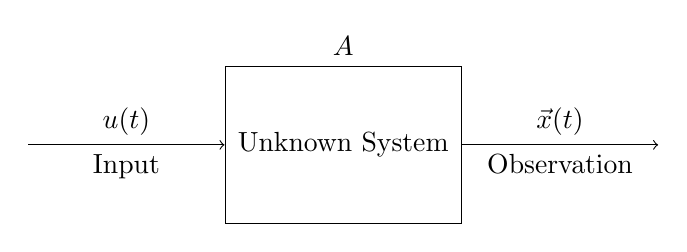
\begin{tikzpicture}
\node[draw, rectangle, minimum width = 3 cm, minimum height = 2 cm] (fl) at (0,0) {Unknown System};
\node[above] at (fl.north) {$A$};
\draw[<-] (fl) -- node[above]{$u(t)$} node[below]{Input} ++(-4,0);
\draw[->] (fl) -- node[above]{$\vec{x}(t)$} node[below]{Observation} ++(4,0);
\end{tikzpicture}
\end{center}

Recall from discussion that if we put a \textbf{piecewise constant} input $u(t) = u(i)$ for $t \in [i, i+1),$ then we can observe the output $\vec{x}(t)$ at time $t = i + 1,$ and form a discretized model of the observation. 

\begin{center}
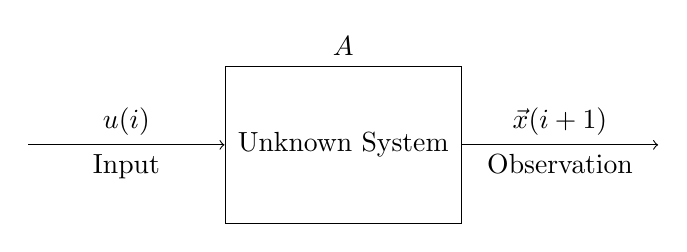
\begin{tikzpicture}
\node[draw, rectangle, minimum width = 3 cm, minimum height = 2 cm] (fl) at (0,0) {Unknown System};
\node[above] at (fl.north) {$A$};
\draw[<-] (fl) -- node[above]{$u(i)$} node[below]{Input} ++(-4,0);
\draw[->] (fl) -- node[above]{$\vec{x}(i + 1)$} node[below]{Observation} ++(4,0);
\end{tikzpicture}
\end{center}

\textbf{If} we knew the system, the relationship between $\vec{x}(i+1), \vec{x}(i),$ and $u(i)$ would be:
\begin{equation}
\vec{x}(i + 1) = A \vec{x}(i) + \vec{b} u(i)
\end{equation}

While this relation is useful, we currently do not know what the $A$ matrix or $\vec{b}$ vector are.

Therefore, we will start by creating unknown variables for the $A$ matrix, and $\vec{b}$ vector:
\begin{equation}
A = \begin{bmatrix} a_{11} & a_{12} \\ a_{21} & a_{22} \end{bmatrix} \ \ \text{and} \ \ \vec{b} = \begin{bmatrix} b_{1} \\ b_{2} \end{bmatrix}
\end{equation}
For the purposes of this question, we will be in the space $\mathbb{R}^2.$

\begin{enumerate}
  \qitem Let's say the system initially started at $\vec{x}(0) = \begin{bmatrix} x_{1}(0) \\ x_{2}(0) \end{bmatrix},$ and we gave an input at time $t = 0, \ u(0).$ 
  At time $t = 1,$ we observe $\vec{x}(1) = \begin{bmatrix} x_{1}(1) \\ x_{2}(1) \end{bmatrix}.$
  \textbf{How can you uncouple this matrix/vector equation into a system of linear equations?}

  \sol {
    We start by writing out the matrix/vector equation for our unknown system:
    \begin{equation}
    \vec{x}(1) = \begin{bmatrix} x_{1}(1) \\ x_{2}(1) \end{bmatrix} = A \vec{x}(0) + \vec{b} u(0) = 
    \begin{bmatrix} a_{11} & a_{12} \\ a_{21} & a_{22} \end{bmatrix} \begin{bmatrix} x_{1}(0) \\ x_{2}(0) \end{bmatrix} + 
    \begin{bmatrix} b_{1} \\ b_{2} \end{bmatrix} u(0)
    \end{equation}

    Uncoupling these equations, we get:
    \pagebreak[0]
    \begin{gather*}
    x_{1}(1) = a_{11} x_{1}(0) + a_{12} x_{2}(0) + b_{1} u(0) \\
    x_{2}(1) = a_{21} x_{1}(0) + a_{22} x_{2}(0) + b_{2} u(0)
    \end{gather*}
  }

  \qitem Based on the system of linear equations created in the previous part, \textbf{how many unknown} variables do we have? Also, if we have a system of linear equations with $n$ unknown variables, at the minimum, \textbf{how many equations} would we need to solve our system?

  \sol {
    The unknowns in this system of linear equations are: $a_{11}, a_{12}, a_{21}, a_{22}, b_{1}, b_{2}.$ \vskip 1pt
    If we have a system of linear equations with $n$ unknown variables, we will need at least $n$ equations to solve the system. 
  }

  \qitem We now give another input at $t = 1, \ u(1),$ and observe $\vec{x}(2).$ \vskip 1pt 
  \textbf{How many more equations do we get from this observation?}
  Also, how many more inputs will we need to observe until we have enough equations?

  \sol {
    We can write out a similar observation as the one made in part(a):
    \begin{equation}
    \vec{x}(2) = \begin{bmatrix} x_{1}(2) \\ x_{2}(2) \end{bmatrix} = A \vec{x}(1) + \vec{b} u(1) = 
    \begin{bmatrix} a_{11} & a_{12} \\ a_{21} & a_{22} \end{bmatrix} \begin{bmatrix} x_{1}(1) \\ x_{2}(1) \end{bmatrix} + 
    \begin{bmatrix} b_{1} \\ b_{2} \end{bmatrix} u(1)
    \end{equation}

    Uncoupling these equations again, we will get:
    \pagebreak[0]
    \begin{gather*}
    x_{1}(2) = a_{11} x_{1}(1) + a_{12} x_{2}(1) + b_{1} u(1) \\
    x_{2}(2) = a_{21} x_{1}(1) + a_{22} x_{2}(1) + b_{2} u(1)
    \end{gather*}
    Notice that for every observation we make at a given time step, we will get $2$ more equations. 
    This means we will have to look at a total of $3$ time steps to get $6$ equations.
    Taking the initial condition $\vec{x}(0)$ into account, we will have to observe a total of $4$ inputs.
  }

  \qitem Assuming we have taken all of the necessary measurements of $x(t)$ at time $t = 0, 1, 2, ...$ \vskip 1pt
  \textbf{How can we set up our system of linear equations as a matrix-vector equation?}

  \sol {
    We can set up the following system of linear equations:
    $$
    \begin{bmatrix}
    x_{1}(0) & x_{2}(0) & u(0) & 0 & 0 & 0 \\
    x_{1}(1) & x_{2}(1) & u(1) & 0 & 0 & 0 \\
    x_{1}(2) & x_{2}(2) & u(2) & 0 & 0 & 0 \\
    0 & 0 & 0 & x_{1}(0) & x_{2}(0) & u(0) \\
    0 & 0 & 0 & x_{1}(1) & x_{2}(1) & u(1) \\
    0 & 0 & 0 & x_{1}(2) & x_{2}(2) & u(2) 
    \end{bmatrix} 
    \begin{bmatrix} a_{11} \\ a_{12} \\ b_{1} \\ a_{21} \\ a_{22} \\ b_{2} \end{bmatrix}
    = \begin{bmatrix} x_{1}(1) \\ x_{1}(2) \\ x_{1}(3) \\ x_{2}(1) \\ x_{2}(2) \\ x_{2}(3) \end{bmatrix}$$
    This can be written in as a matrix vector equation $D \vec{s} = \vec{y}$ and we can solve for $\vec{s} = D^{-1} \vec{y}$  
  }

  \qitem While we can set up a matrix vector equation and uniquely solve our system, the output of the system can be noisy.
  Therefore, we update our model by considering a noise term $w(i)$ at time $t = i.$
  \begin{equation}
    \vec{x}(i + 1) = A \vec{x}(i) + \vec{b} u(i) + w(i)
  \end{equation}
  How can we set up a system of equations in a similar fashion but with a noise vector $\vec{w}?$
  \begin{equation}
    \vec{y} = D \vec{s} + \vec{w}
  \end{equation}

  \sol {
    $$
    \begin{bmatrix} x_{1}(1) \\ x_{1}(2) \\ x_{1}(3) \\ x_{2}(1) \\ x_{2}(2) \\ x_{2}(3) \end{bmatrix} 
    = 
    \begin{bmatrix}
    x_{1}(0) & x_{2}(0) & u(0) & 0 & 0 & 0 \\
    x_{1}(1) & x_{2}(1) & u(1) & 0 & 0 & 0 \\
    x_{1}(2) & x_{2}(2) & u(2) & 0 & 0 & 0 \\
    0 & 0 & 0 & x_{1}(0) & x_{2}(0) & u(0) \\
    0 & 0 & 0 & x_{1}(1) & x_{2}(1) & u(1) \\
    0 & 0 & 0 & x_{1}(2) & x_{2}(2) & u(2) 
    \end{bmatrix} 
    \begin{bmatrix} a_{11} \\ a_{12} \\ b_{1} \\ a_{21} \\ a_{22} \\ b_{2} \end{bmatrix}
    + \begin{bmatrix} w(0) \\ w(1) \\ w(2) \\ w(0) \\ w(1) \\ w(2) \end{bmatrix} $$
  }

  \qitem We can try to solve our system of equations, but we do not know what $\vec{w}$ is. \vskip 1pt
  What we can do however, is to take more measurements, and set up a \textbf{least squares} problem as seen in 16A.
  What would the least squares problem be if we took measurements up to time step $t = 5?$ 

  \sol {
  $$
    \begin{bmatrix} x_{1}(1) \\ x_{1}(2) \\ x_{1}(3) \\ x_{1}(4) \\ x_{1}(5) \\ x_{2}(1) \\ x_{2}(2) \\ x_{2}(3) \\ x_{2}(4) \\ x_{2}(5) \end{bmatrix} 
    = 
    \begin{bmatrix}
    x_{1}(0) & x_{2}(0) & u(0) & 0 & 0 & 0 \\
    x_{1}(1) & x_{2}(1) & u(1) & 0 & 0 & 0 \\
    x_{1}(2) & x_{2}(2) & u(2) & 0 & 0 & 0 \\
    x_{1}(3) & x_{2}(3) & u(3) & 0 & 0 & 0 \\
    x_{1}(4) & x_{2}(3) & u(4) & 0 & 0 & 0 \\
    0 & 0 & 0 & x_{1}(0) & x_{2}(0) & u(0) \\
    0 & 0 & 0 & x_{1}(1) & x_{2}(1) & u(1) \\
    0 & 0 & 0 & x_{1}(2) & x_{2}(2) & u(2) \\
    0 & 0 & 0 & x_{1}(3) & x_{2}(3) & u(3) \\
    0 & 0 & 0 & x_{1}(4) & x_{2}(4) & u(4) 
    \end{bmatrix} 
    \begin{bmatrix} a_{11} \\ a_{12} \\ b_{1} \\ a_{21} \\ a_{22} \\ b_{2} \end{bmatrix}
    + \begin{bmatrix} w(0) \\ w(1) \\ w(2) \\ w(0) \\ w(1) \\ w(2) \end{bmatrix} $$

    Which can equivalently be written as:
    \begin{equation}
      \vec{y} = D \vec{s} + \vec{w}
    \end{equation}
    For the least squares problem, we will want to minimize $\norm{\vec{w}}_{2} = \norm{y - D \vec{s}}_{2}$
    }

  \qitem How would we solve this least squares problem?

  \sol {
    Recall from 16A that if we are given the least squares problem:
    \begin{equation}
      A \vec{x} = \vec{b} + \vec{e}
    \end{equation}
    The solution that minimizes the norm of the residual $\norm{\vec{e}}_{2}$ is:
    \begin{equation}
      \vec{\hat{x}} = (A^{T} A)^{-1} A^{T} \vec{b}
    \end{equation}
    Therefore the solution to the least squares problem above will be:
    \begin{equation}
      \vec{\hat{s}} = (D^{T} D)^{-1} D^{T} \vec{y}
    \end{equation}
    The $\vec{\hat{s}}$ will give the best possible estimate for the $A$ and $\vec{b}.$
  }
\end{enumerate}


% \newpage
% % Author: Taejin Hwang
% Email: taejin@berkeley.edu

\qns{Controlling a System}

We are given a discrete time state space system, where $\vec{x}$ is our \textbf{state vector,} $A$ is the state space \textbf{model}, $B$ is the input \textbf{matrix}, and $\vec{u}$ is the control input \textbf{vector.}
\begin{equation}
\vec{x}(t + 1) = A \vec{x}(t) + B\vec{u}(t)
\end{equation}
We want to know if this system is “controllable”; if given set of inputs, we can get the system from any initial state to any final state. This has an important physical meaning; if a physical system is controllable, that means that we can get anywhere in the state space. If a robot is controllable, it is able to travel anywhere in the system it is living in (given enough control inputs).

We will start with the assumption that the system started at rest: $\vec{x}(0) = \vec{0},$ and our state space will be $\mathbb{R}^{n}.$ 

\begin{enumerate}

\qitem How can you write out $\vec{x}(1)$ using the state space equation? How about $\vec{x}(2)?$

\sol {
  Using the state space model $\vec{x}(t + 1) = A \vec{x}(t) + B \vec{u}(t),$
  $$\vec{x}(1) = A \vec{x}(0) + B \vec{u}(0) = A \vec{0} + B \vec{u}(0) = B \vec{u}(0)$$
  At time step $t = 2,$
  $$\vec{x}(2) = A \vec{x}(1) + B \vec{u}(1) = A (B \vec{u}(0)) + B \vec{u}(1)$$
}

\qitem Given these two observations, where in our state space can $\vec{x}$ reach at time $t = 2?$

\sol {
  From the previous part, we know that
  $$\vec{x}(2) = A (B \vec{u}(0)) + B \vec{u}(1) = AB \vec{u}(0) + B \vec{u}(1)$$
  Let's say $B$ has two columns, although we can generalize this for any number of columns. \vskip 1pt
  We can then equivalently write out our equation as:
  $$\vec{x}(2) = \begin{bmatrix} A \vec{b}_{1} & A \vec{b}_{2} \end{bmatrix} \begin{bmatrix} u_{1}(0) \\ u_{2}(0) \end{bmatrix} + 
  \begin{bmatrix} \vec{b}_{1} & \vec{b}_{2} \end{bmatrix} \begin{bmatrix} u_{1}(1) \\ u_{2}(1) \end{bmatrix} = 
  u_{1}(0) A \vec{b}_{1} + u_{2}(0) A \vec{b}_{2} + u_{1}(1) \vec{b}_{1} + u_{2}(1) \vec{b}_{2}.$$
  Since $\vec{u}$ is a vector we have full control over, we can reach anywhere in:
  $$\text{span}(A \vec{b}_{1}, A \vec{b}_{2}, \vec{b}_{1}, \vec{b}_{2})$$
  In general, we could reach anywhere in the span of the columns of $B$ and $AB.$
}

\qitem Given these $n$ observations, where in our state space can $\vec{x}$ reach at time $t = n?$

\sol {
  We will start off in a similar manner by writing out $\vec{x}(3)$ in terms of $\vec{x}(2)$ and $\vec{u}(2).$
  $$\vec{x}(3) = A \vec{x}(2) + B \vec{u}(2) =  A (AB \vec{u}(0) + B \vec{u}(1)) + B \vec{u}(2) = A^2 B \vec{u}(0) + AB \vec{u}(1) + B \vec{u}(2).$$
  Using a similar argument as the previous part, we will see that we can reach anywhere in the span of the columns of $B, \ AB, \ A^{2} B.$ We can continue doing this, and see that after $n$ time steps,
  \begin{align*}
  \vec{x}(n) &= A \vec{x}(n - 1) + B \vec{u}(n - 1) \\
  &= A^{n - 1}B \vec{u}(0) + A^{n - 2}B \vec{u}(1) + A^{n - 3}B \vec{u}(2) + \cdots + AB \vec{u}(n - 2) + B \vec{u}(n - 1)
  \end{align*}
  Therefore, after $n$ timesteps, we can reach anywhere in the span of the columns of $\{ B, \ AB, \ A^2 B, \cdots, A^{n-1} B \}.$
}

\qitem Show that if the columns of $A^{k} B$ are linearly dependent, then the columns of $A^{k + 1} B$ are also linearly dependent.

\sol {
  We first make the observation that the columns of $A^{k} B$ are:
  $$A^{k} B = \begin{bmatrix} A^{k} \vec{b_1} & A^{k} \vec{b_2} & \cdots & A^{k} \vec{b_m} \end{bmatrix}$$
  Where $\vec{b}_{i}$ is the $i^{th}$ column of the matrix $B.$ \vskip 1pt
  Now let's suppose that the columns of $A^{k} B$ are linearly independent, then we can say that if we have scalars $\alpha_i$ such that 
  $$\alpha_{1} A^{k} \vec{b_1} + \cdots + \alpha_{m} A^{k} \vec{b_m} = \vec{0},$$
  then at least one of the $\alpha_i$ must be nonzero. Now if we left multiply by $A,$ we see that:
  $$A(\alpha_{1} A^{k} \vec{b_1} + \cdots + \alpha_{m} A^{k} \vec{b_m}) = \alpha_{1} A^{k+1} \vec{b_1} + \cdots + \alpha_{m} A^{k+1} \vec{b_m} = \vec{0}.$$ 
  As a result, we observe that if we have a linear combination of the columns of $A^{k + 1} B$ equal to the zero vector, at least one of the scalars is nonzero, meaning the columns of $A^{k + 1} B$ must be linearly dependent.
}

\qitem To summarize our work from the previous parts, we now define a controllability matrix

\meta {
  This is definitely the most difficult part of the question, the previous parts were more or less intuitive, but here students will have to think about how part (d) relates to "redundant" measurements.
}

\begin{equation}
\mathcal{C} = \begin{bmatrix} B & AB & A^2B & \cdots & A^{n-2}B & A^{n-1}B \end{bmatrix}
\end{equation}
Based on the previous parts, when can we say our system is "controllable," it can reach anywhere in our state space? 

\sol {
  Using our knowledge from part (c), we can say that $\vec{x}$ can reach anywhere in the span of the columns of $\mathcal{C}$ after $n$ time steps. 
  We also saw in part (d), that if $A^{k}B$ had linearly dependent columns, then $A^{k + 1}B$ will also have linearly dependent columns. \vskip 1pt
  This means if one of our measurements at time $t = k,$ were linearly dependent from our previous measurements, then the future measurements $t = k + 1$ onward, will also be linearly dependent from the previous ones. In other words, every redundant measurement taken after a redundant one will continue to be redundant. \vskip 1pt
  We must take at least $n$ measurements, since we want to span all of $\mathbb{R}^n,$ and $B$ may just be a single vector.
  Therefore, we conclude by saying that our system can reach anywhere in our state-space, $\mathbb{R}^{n},$ if $\mathcal{C}$ is a matrix of rank $n.$ \vskip 1pt
  This does not mean that $\mathcal{C}$ has to be invertible, it just means that $\mathcal{C}$ must have $n$ linearly independent columns for the system to be controllable.
}

\end{enumerate}
% \newpage
% \qns{Controllability Practice}

Consider the system 
\[\vec{x}(t + 1) = 
\begin{bmatrix}
    0 & 1 & -2 \\
    0 & 2 & 0 \\
    -1 & 1 & 0
\end{bmatrix} \vec{x}(t) + 
\begin{bmatrix}
    2 \\ 0 \\ 0
\end{bmatrix} u(t)\]

\begin{enumerate}
    \qitem \textbf{What is the controllability matrix, $\mathcal{C}$, for this system?}
    \ws{\vspace{100px}}
    \sol{
        For a 3-dimensional system,
        \[\mathcal{C} = 
        \begin{bmatrix}
            \vec{b} & A\vec{b} & A^2 \vec{b}
        \end{bmatrix}\]
        Plugging in this system's $A$ and $\vec{b}$, we have
        \[\mathcal{C} = 
        \begin{bmatrix}
            2 & 0 & 4 \\
            0 & 0 & 0 \\
            0 & -2 & 0
        \end{bmatrix}\]
        The column space of $\mathcal{C}$ is the span of its column vectors. 
        The third column is linearily dependent, so $\text{col}(\mathcal{C})$ is equivalent to the span of its first two columns.
        \[\text{col}(\mathcal{C}) = \text{span}\{ \begin{bmatrix} 1 \\ 0 \\ 0 \end{bmatrix}, \begin{bmatrix} 0 \\ 0 \\ 1 \end{bmatrix}\}\]
    }

    \qitem \textbf{What is the rank of the controllability matrix? Is the system controllable?}

    \ws{\vspace{75px}}

    \sol{
        The controllability matrix has rank 2, so this system is not controllable.
        Note that the initial state $\vec{x}(0)$ has no effect on whether a system is controllable.
    }

    \qitem \textbf{Starting at $\vec{x}(0) = \begin{bmatrix} 1 \\ 0 \\ 0 \end{bmatrix}$, what possible states can we reach after one timestep? Two timesteps? Three?}
    
    \ws{\vspace{150px}}

    \sol{
        For one timestep,
        \[\vec{x}(1) = 
        \begin{bmatrix}
            0 & 1 & -2 \\
            0 & 2 & 0 \\
            -1 & 1 & 0
        \end{bmatrix} 
        \begin{bmatrix} 
            1 \\ 0 \\ 0 
        \end{bmatrix}
        + \begin{bmatrix}
            2 \\ 0 \\ 0
        \end{bmatrix} u(0)\]

        Simplifying, we get
        \[\vec{x}(1) =
        \begin{bmatrix} 
            0 \\ 0 \\ -1 
        \end{bmatrix} + 
        \begin{bmatrix} 
            2u(0) \\ 0 \\ 0 
        \end{bmatrix} = 
        \begin{bmatrix} 
            2u(0) \\ 0 \\ -1 
        \end{bmatrix}\]

        Since $u(0)$ is an input we have control over, we can set it arbitrarily, and reach any state of the form 
        \[ \begin{bmatrix} c_1 \\ 0 \\ -1\end{bmatrix}. \]
        For two timesteps,
        \[\vec{x}(2) = 
        \begin{bmatrix}
            0 & 1 & -2 \\
            0 & 2 & 0 \\
            -1 & 1 & 0
        \end{bmatrix} 
        \begin{bmatrix} 
            2u(0) \\ 0 \\ -1
        \end{bmatrix}
        + \begin{bmatrix}
            2 \\ 0 \\ 0
        \end{bmatrix} u(1) = 
        \begin{bmatrix} 
            2 + 2u(1) \\ 0 \\ -2u(0)
        \end{bmatrix}\]
        Again, since we have control over $u(0)$ and $u(1)$, we can reach any state of the form $\begin{bmatrix} c_1 \\ 0 \\ c_2 \end{bmatrix}$. \\
        \newline
        For 3 timesteps,
        \[\vec{x}(3) = 
        \begin{bmatrix}
            0 & 1 & -2 \\
            0 & 2 & 0 \\
            -1 & 1 & 0
        \end{bmatrix} 
        \begin{bmatrix} 
            2 + 2u(1) \\ 0 \\ -2u(0)
        \end{bmatrix}
        + \begin{bmatrix}
            2 \\ 0 \\ 0
        \end{bmatrix} u(2) = 
        \begin{bmatrix} 
            4u(0) + 2u(2) \\ 0 \\ -2 - 2u(1)
        \end{bmatrix}\]
        As with 2 timesteps, we can reach any state of the form $\begin{bmatrix} c_1 \\ 0 \\ c_2 \end{bmatrix}$.
    }

    \qitem \textbf{What is the minimum number of timesteps it takes to reach $\begin{bmatrix} 1 \\ 0 \\ 2 \end{bmatrix}$? 
    What about $\begin{bmatrix} 1 \\ 1 \\ 1 \end{bmatrix}$?}

    \ws{\vspace{100px}}

    \sol{
        It takes two timesteps to reach $\begin{bmatrix} 1 \\ 0 \\ 2 \end{bmatrix}$. \\
        $\begin{bmatrix} 1 \\ 0 \\ 2 \end{bmatrix}$ is in the form $\begin{bmatrix} c_1 \\ 0 \\ c_2 \end{bmatrix}$, but not in the form $\begin{bmatrix} c_1 \\ 0 \\ -1 \end{bmatrix}$, so it can be reached in at least two timesteps. \\
        \newline
        It is impossible to reach $\begin{bmatrix} 1 \\ 1 \\ 1 \end{bmatrix}$ in any amount of timesteps.
        The system is not controllable, and we can only reach states of the form $\begin{bmatrix} c_1 \\ 0 \\ c_2 \end{bmatrix}$.
    }
\end{enumerate}

Now, consider the system, with $A$ modified slightly:
\[\vec{x}(t + 1) = 
\begin{bmatrix}
    0 & 1 & 0 \\
    0 & 2 & -2 \\
    -1 & 1 & 0
\end{bmatrix} \vec{x}(t) + 
\begin{bmatrix}
    2 \\ 0 \\ 0
\end{bmatrix} u(t)\]

\begin{enumerate}[resume]
  \qitem \textbf{What is the controllability matrix, $\mathcal{C}$, for this system? What is its column space?}
  \ws{\vspace{100px}}
  \sol {
    \[\mathcal{C} = 
    \begin{bmatrix}
        \vec{b} & A\vec{b} & A^2 \vec{b}
    \end{bmatrix} = 
    \begin{bmatrix}
        2 & 0 & 0 \\
        0 & 0 & 4 \\
        0 & -2 & 0
    \end{bmatrix}\]
    The column space of this matrix spans $\mathbb{R}^3$.
  }

  \qitem \textbf{What is the rank of the controllability matrix? Is the system controllable?}

  \ws{\vspace{50px}}
  \sol {
    The controllability matrix has rank 3, so the system is controllable.
  }

  \qitem \textbf{Starting at $\vec{x}(0) = \begin{bmatrix} 1 \\ 0 \\ 0 \end{bmatrix}$, what possible states can we reach after one timestep? Two timesteps? Three?}

  \ws{\vspace{100px}}
  \sol {
    For one timestep, 
    \[\vec{x}(1) = 
    \begin{bmatrix}
        0 & 1 & 0 \\
        0 & 2 & -2 \\
        -1 & 1 & 0
    \end{bmatrix} 
    \begin{bmatrix} 
        1 \\ 0 \\ 0 
    \end{bmatrix}
    + \begin{bmatrix}
        2 \\ 0 \\ 0
    \end{bmatrix} u(0) =
    \begin{bmatrix} 
        2u(0) \\ 0 \\ -1 
    \end{bmatrix}\]
    So, we can reach any state of the form $\begin{bmatrix} c_1 \\ 0 \\ -1 \end{bmatrix}$. \\
    \newline

    For two timesteps,
    \[\vec{x}(2) = 
    \begin{bmatrix}
        0 & 1 & 0 \\
        0 & 2 & -2 \\
        -1 & 1 & 0
    \end{bmatrix} 
    \begin{bmatrix} 
        2u(0) \\ 0 \\ -1 
    \end{bmatrix}
    + \begin{bmatrix}
        2 \\ 0 \\ 0
    \end{bmatrix} u(1) =
    \begin{bmatrix} 
        2u(1) \\ 2 \\ -2u(0) 
    \end{bmatrix}\]
    We can reach any state of the form $\begin{bmatrix} c_1 \\ 2 \\ c_2 \end{bmatrix}$. \\
    \newline

    For three timesteps,
    \[\vec{x}(3) = 
    \begin{bmatrix}
        0 & 1 & 0 \\
        0 & 2 & -2 \\
        -1 & 1 & 0
    \end{bmatrix} 
    \begin{bmatrix} 
        2u(1) \\ 2 \\ -2u(0) 
    \end{bmatrix}
    + \begin{bmatrix}
        2 \\ 0 \\ 0
    \end{bmatrix} u(2) =
    \begin{bmatrix} 
        2 + 2u(2) \\ 4 + 4u(0) \\ 2 - 2u(1) 
    \end{bmatrix}\] 
    We can reach any state in $\mathbb{R}^3$ in three timesteps.
  }

  \qitem \textbf{What is the minimum number of timesteps it takes to reach $\begin{bmatrix} 1 \\ 0 \\ 2 \end{bmatrix}$?} \\
    \textit{Hint: 
      Since the system is controllable, we can reach any state in three time steps, however, it may be possible to reach a state in fewer than three time steps. Look at your answer to the previous part, and check which possible states we can reach in one, two, and three time steps.
    }

  \ws{\vspace{50px}}
    
  \sol {
    We unfortunately cannot reach this vector in fewer timesteps because $\begin{bmatrix} 1 \\ 0 \\ 2 \end{bmatrix}$ is not in the form $\begin{bmatrix} c_1 \\ 0 \\ -1 \end{bmatrix}$ or $\begin{bmatrix} c_1 \\ 2 \\ c_2 \end{bmatrix}.$
  }

  \qitem \textbf{What is the minimum number of timesteps it takes to reach $\begin{bmatrix} 1 \\ 2 \\ 3 \end{bmatrix}$?}
  \ws{\vspace{50px}}
  \sol {
    We can reach this vector in two time steps since it is in the form $\begin{bmatrix} c_1 \\ 0 \\ -1 \end{bmatrix}$ or $\begin{bmatrix} c_1 \\ 2 \\ c_2 \end{bmatrix}.$
  }

\end{enumerate}
% \newpage	
% % Authors: Taejin Hwang, Justin Yu
% Emails: taejin@berkeley.edu, justinvyu@berkeley.edu

\qns{Inner Products and Orthogonality}

We are very familiar with how to add vectors and multiply them with a scalar, but we never defined how to multiply two vectors.

An \textbf{inner product} over the real numbers, is a rule that takes two vectors $\vec{x}, \vec{y} \in V$ and outputs a scalar in $\mathbb{R}$ that satisfies the following properties:

\meta {
  Note that the properties below are for $\textbf{real}$ inner products, and \textbf{complex} inner products will be covered later on in 16B.
}

\begin{enumerate}[label=(\roman*)]
  \item Symmetry: $\innp{\vec{x}}{\vec{y}} = \innp{\vec{y}}{\vec{x}}$
  \item Homogeneity: $\innp{\alpha \vec{x}}{\vec{y}} = \alpha \innp{\vec{x}}{\vec{y}}$
  \item Additivity: $\innp{\vec{x}+\vec{y}}{\vec{z}} = \innp{\vec{x}}{\vec{z}} + \innp{\vec{y}}{\vec{z}}$
  \item Positive-definiteness: $\innp{\vec{x}}{\vec{x}} \geq 0$, and is $= 0$ iff $\vec{x} = \vec{0}$
\end{enumerate}

In this question, we will review the concepts of an inner product, and focus our attention on when two vectors are \textbf{orthogonal}. We say two vectors $\vec{x}$ and $\vec{y}$ are orthogonal if:
\begin{equation}
  \langle \vec{x}, \vec{y} \rangle = 0
\end{equation}

If we plotted these vectors geometrically, then the two vectors would appear to be perpendicular.
\begin{enumerate}
  \qitem What is the difference between a dot product and an inner product?
  
  \meta {
    The purpose of this part is to make sure students understand that not all inner products are the dot product, since they will see examples of 
  }

  \sol {
    A dot product is a special case of the inner product in $\mathbb{R}^{n}$ where:
    \begin{equation}
      \innp{\vec{x}}{\vec{y}} = \vec{x}^{T} \vec{y}
    \end{equation}
    An inner product is a generalization in which we multiply two vectors in a vector space that satisfies the four properties above.
    We will take a look at other inner products that are not necessarily the dot product, in 16B.
  }

  \qitem We can define the \textbf{norm} of a vector using an inner product. 
  The \textbf{Euclidean norm} is defined as:
  \begin{equation}
    \norm{\vec{x}} = \sqrt{\innp{\vec{x}}{\vec{x}}}
  \end{equation}
  Recall the cosine definition of a dot product using norms, where $\theta$ is the angle between $\vec{x}$ and $\vec{y}$:
  \begin{equation}
    \vec{x} \cdot \vec{y} = \norm{\vec{x}} \norm{\vec{y}} \cos(\theta)
  \end{equation}
  Show that if $\vec{x}$ and $\vec{y}$ are non-zero and orthogonal, then the angle between the two vectors is $90^{\circ}.$

  \sol {
    If $\vec{x}$ and $\vec{y}$ are orthogonal, then their inner product must be zero.
    $$\innp{\vec{x}}{\vec{y}} = 0.$$
    This means that $\norm{\vec{x}} \norm{\vec{y}} \cos(\theta) = 0.$ Since $\vec{x}, \vec{y} \neq \vec{0},$ $\norm{\vec{x}}, \norm{\vec{y}}$ must be non-zero, which implies that $\cos(\theta) = 0.$
    We conclude by saying that $\theta = \frac{\pi}{2}$ or $90^{\circ}.$
  }

  \qitem Show that $\vec{0}$ is orthogonal to any vector $\vec{x} \in \mathbb{R}^{n}$ using the definition of the dot product.

  \sol {
    $$\vec{x} \cdot \vec{0} = \vec{x}^{T} \vec{0} = x_{1} \cdot 0 + \cdots x_{n} \cdot 0 = 0.$$
  }

  \qitem Show that if $\vec{v}_{1}$ and $\vec{v}_{2}$ are non-zero and orthogonal, then they must be linearly independent.

  \sol {
    We must show that if $\alpha_{1} \vec{v}_{1} + \alpha_{2} \vec{v}_{2} = \vec{0},$ then $\alpha_{1} = \alpha_{2} = 0.$ \vskip 1pt
    We start off by taking the inner product of both sides with $\vec{v}_{1}$
    $$\innp{\alpha_{1} \vec{v}_{1} + \alpha_{2} \vec{v}_{2}}{\vec{v}_{1}} = \innp{\vec{0}}{\vec{v}_{1}}$$
    Using the scaling and additivity properties of the inner product, we see that:
    $$\alpha_{1} \innp{\vec{v}_{1}}{\vec{v}_{1}} + \alpha_{2} \innp{\vec{v}_{2}}{\vec{v}_{1}} = \innp{\vec{0}}{\vec{v}_{1}}$$
    We know that $\vec{0}$ and $\vec{v}_{2}$ are both orthogonal to $\vec{v}_{1}$ so their inner products must be $0.$
    $$\alpha_{1} \innp{\vec{v}_{1}}{\vec{v}_{1}} = 0.$$
    We also know that $\vec{v}_{1}$ is non-zero so $\norm{\vec{v}_{1}} > 0.$
    Which implies that $\alpha_{1}$ must be zero. \vskip 1pt
    The exact same argument can be used one more time, by taking the inner product of both sides with $\vec{v}_{2}$ to show that $\alpha_{2}$ must also be zero, which shows that $\vec{v}_{1}$ and $\vec{v}_{2}$ must be linearly independent.
  }

  \qitem Generalize the argument above to show that if $\{\vec{v}_{1}, \cdots, \vec{v}_{n}\}$ is a set of non-zero orthogonal vectors, then the set must be linearly independent. 
  We say a set of vectors is orthogonal, if each pair of vectors is mutually orthogonal, that is $\innp{\vec{v}_{i}}{\vec{v}_{j}} = 0$ for any $i,j$ where $i \neq j.$

  \meta {
    If students aren't comfortable with summations, especially the $1 \leq i < j \leq n$ part, then use the first method provided in the solution.
  }

  \sol {
    The argument should almost be identical. We must show that if $\alpha_{1} \vec{v}_{1} + \cdots + \alpha_{n} \vec{v}_{n} = \vec{0},$ then $\alpha_{1} = \hdots = \alpha_{n} = 0.$ We can use the same argument by taking the inner product of both sides with $\vec{v}_{1}$
    to show that $\alpha_{1}$ is zero, and then generalize it for all $i = \{1, \hdots, n \}.$ \vskip 1pt
    However, another clever way to do this problem is to take the inner product of both sides with itself:
    $$\innp{\alpha_{1} \vec{v}_{1} + \cdots + \alpha_{n} \vec{v}_{n}}{\alpha_{1} \vec{v}_{1} + \cdots + \alpha_{n} \vec{v}_{n}} = \innp{\vec{0}}{\vec{0}}$$ 
    Again we use the distributive properties of additivity and scaling to see that:
    $$\sum\limits_{i = 1}^{n} \alpha_{i}^{2} \innp{\vec{v}_{i}}{\vec{v}_{i}} \ + \ \sum\limits_{1 \leq i < j \leq n} \alpha_{i} \alpha_{j} \innp{\vec{v}_{i}}{\vec{v}_{j}} \ + \ \sum\limits_{1 \leq j < i \leq n} \alpha_{i} \alpha_{j} \innp{\vec{v}_{j}}{\vec{v}_{i}} = \innp{\vec{0}}{\vec{0}}$$ 
    Since the vectors are all mutually orthogonal, we see that:
    $$\sum\limits_{i = 1}^{n} \alpha_{i}^{2} \innp{\vec{v}_{i}}{\vec{v}_{i}} = 0$$
    Since all of the vectors $\vec{v}_{i}$ are non-zero, $\norm{\vec{v}_{i}} > 0.$ In addition, all of the scalars, $\alpha_{i}^{2}$ are greater than or equal to zero.
    However, since the linear combination is still equal to $0,$ all of the $\alpha_{i}$ must be equal to $0$ meaning the set is linearly independent.
  }
\end{enumerate}




% \qns{Spectral Norm Proof} 
\qcontributor{Anant Sahai}
\qcontributor{Elena Jia}


Given a matrix $A \in \mathbb{R}^{m,n}$ of rank $r$ with singular values $\sigma_{1} \geq \sigma_{2} \geq \cdots \geq \sigma_{r} > \sigma_{r+1} = \cdots = \sigma_{n} = 0$. 
We want to show that 
\begin{equation}
\norm{A}_{2} = \max_{\vec{x} \neq \vec{0}} \frac{\|A\vec{x}\|}{\|\vec{x}\|} = \sigma_{1}
\end{equation} where $\norm{A}_{2}$ is the spectral norm of $A$ and $\vec{x} \in \mathbb{R}^{n}$ (i.e.~that the maximum factor by which that $A$ can grow the Euclidean norm is $\sigma_1$). 
% Since matrix $A^{T}A$ is symmetric, we know $A^{T}A$ has eigenvalue decomposition $VSV^{T}.$ Let $v_{1}, v_{2}, ..., v_{n}$ be the set of orthonormal eigenvectors of $A^{T}A$ with associated eigenvalues $\lambda_{1} \geq \lambda_{2} \geq ... \geq \lambda_{n} $ .

We start by noting that since the matrix $A^{T}A$ is symmetric, we know $A^{T}A$ has eigenvalue decomposition $V \Lambda V^{T}.$ Let $\vec{v}_{1}, \vec{v}_{2}, \ldots, \vec{v}_{n}$ be a set of orthonormal eigenvectors of $A^{T}A$ with associated eigenvalues $\lambda_{1} \geq \lambda_{2} \geq \cdots \geq \lambda_{n}$, where $\lambda_i = \sigma_i^2$.


\begin{enumerate}

% \qitem First, explain why matrix $A^{T}A$ is symmetric and write out the eigenvalue decomposition of $A^{T}A$.
% \sol {
% }

\qitem For $x \in \mathbb{R}^{n}$, decompose $x$ as a linear combination of the set of orthonormal eigenvectors of $A^{T}A$. Then, \textbf{express $\|Ax\|_{2}^{2}$ in terms of $v_{i}$, $x$, and $\sigma_{i}$}, for $i \in \{1, 2, ...,n\}.$

\sol {
Since the eigenvectors are orthonormal, we have $$x = \sum_{i=1}^{n} \langle x,v_i \rangle v_i. $$
Therefore,
		\begin{align} \|Ax\|_{2}^2  
			&= (Ax)^TAx \\
			&= x^TA^TAx \\
			&= \sum_{i=1}^n \lambda_i \langle x,v_i \rangle^2
        \end{align}
Since $$ A^TA = (USV^T)^T(USV^T) = VS^2V^T$$, the eigenvalues of $A^TA$ satisfy $\lambda_i = \sigma_i ^2.$
So we can express $$\|Ax\|_{2}^{2} = \sum_{i=1}^{n} \sigma_i ^2  \langle x,v_i \rangle^2 $$
}

\qitem \textbf{Find a unit vector $x$ that maximizes $\|Ax\|_{2}^{2}.$}

\sol {
  Since $x$ is a unit vector, we know 
  \begin{align} 1 &= \|x\|^{2} \\
  & = \Big(\sum_{i=1}^{n} \langle x,v_i \rangle v_i\Big)^T\Big(\sum_{i=1}^{n}\langle x,v_i \rangle v_i\Big)\\
  & = \sum_{i=1}^{n} \langle x,v_i \rangle ^2 \\
  \end{align}
  Thus, the maximum of $\|Ax\|^{2}$ satisfies $$ 
  	\max \|Ax\|_{2}^{2} = \max \sum_{i=1}^{n} \sigma_i ^2  \langle x,v_i \rangle^2  = \sigma_1 ^2 $$ with the maximum reached when $\langle x,v_1 \rangle^2 = 1$ and $ \langle x,v_j \rangle^2 = 0$ for $j \neq 1$. This gives the unit vector $$ x = \sum_{i=1}^{n}\langle x,v_i\rangle v_i = \pm v_1$$
}

\qitem \textbf{Show that $\|Ax\|_{2} \leq \sigma_{1} \|x\|_{2}$ for any $x \in \mathbb{R}^{n}$.} Thus, $\max \frac{\|Ax\|_{2}}{\|x\|_{2}} = \sigma_{1}.$

\sol {

From previous parts, we know 
\begin{align} \|Ax\|_{2}^{2} &= \sum_{i=1}^{n} \sigma_i ^2  \langle x,v_i \rangle^2 \\
	&\leq \sigma_1^2  \sum_{i=1}^{n} \langle x,v_i \rangle^2 \\
	&= \sigma_1^2 \|x\|^{2}.
\end{align}
Thus, $$\|Ax\|_{2} \leq \sigma_{1} \|x\|_{2}.$$ 

And when $x=\pm \|x\|v_1$, the maximum of $\frac{\|Ax\|_{2}}{\|x\|_{2}}$ is reached: $$\max \frac{\|Ax\|_{2}}{\|x\|_{2}} = \sigma_{1}.$$
  
}






\end{enumerate}

% \newpage

% % Author: Taejin Hwang

\qns{The Frobenius Inner Product}

We previously defined inner products as a way to multiply two vectors to get a scalar and saw numerous examples of the inner product used in $\mathbb{R}^{n}.$

We will now define a new inner product for the vector space of $m \times n$ matrices: $\mathbb{R}^{m \times n}.$
Note that vectors in this space, are in fact $m \times n$ matrices!
We call this inner product the \textbf{Frobenius Inner Product} defined as:
\begin{equation}
  \innp{A}{B}_{F} = \text{Trace}(A^{T} B)
\end{equation}
The trace of a square matrix is the sum of all of its entires along its diagonal.

Similar to how we defined a norm for vectors, we can also define the Frobenius norm for matrices in $\mathbb{R}^{m \times n}\ $as:
\begin{equation}
  \norm{A}_{F} = \sqrt{\innp{A}{A}_{F}} = \sqrt{\text{Trace}(A^{T} A)} = \sqrt{\text{Trace}(A A^{T})}
\end{equation}

In this question, we will investigate into the Frobenius norm, and its relation to the SVD.

\begin{enumerate}
  \item Let $A$ be an $m \times n$ matrix, and $U$ be a square matrix with orthonormal columns. Show that $\norm{UA}_{F} = \norm{A}_{F.}$

  \sol {
    $$\norm{UA}_{F} = \sqrt{\text{Trace}((UA)^{T} (UA))} = \sqrt{\text{Trace}(A^{T} U^{T} (UA))} = \sqrt{\text{Trace}(A^{T} A)} = \norm{A}_{F}.$$
  }

  \item Now let $V$ be another square matrix with orthonormal columns. Show that $\norm{AV}_{F} = \norm{A}_{F}.$

  \sol {
    $$\norm{AV}_{F} = \sqrt{\text{Trace}((AV)(AV)^{T})} = \sqrt{\text{Trace}(AVV^{T} A^{T})} = \sqrt{\text{Trace}(A A^{T})} = \norm{A}_{F}.$$
  }

  \item Use the two facts above to show that $\norm{A}_{F} = \norm{\Sigma}.$

  \sol {
    We know from the SVD that $A = U \Sigma V^{T}$ therefore, $\norm{A}_{F} = \norm{U \Sigma V^{T}}.$
    Since $U$ and $V^{T}$ are both square matrices with orthonormal columns, it follows that $\norm{A}_{F} = \norm{\Sigma}_{F}.$
  }

  \item Conclude by saying that $\norm{A}_{F} = \sqrt{\sum\limits_{i = 1}^{n} \sigma_{i}^{2}}.$

  \sol {
    $\norm{A}_{F} = \norm{\Sigma}_{F} = \sqrt{\text{Trace}(\Sigma^{T} \Sigma)}.$ \\
    Since $\Sigma^{T} \Sigma$ is a diagonal matrix, it follows that $\norm{A}_{F} = \sqrt{\sum\limits_{i = 1}^{n} \sigma_{i}^{2}}.$
  }

\end{enumerate}
% \newpage
% % Author: Taejin Hwang

\qns{Low Rank Approximation}

Given a $m \times n$ matrix $A,$ of high rank, we want to see how we can best approximate this matrix $A$ using a lower rank matrix $A_{k}$ of rank $k << n.$ 

Before we do this however, we will need to define a way to measure how large a matrix is, and how good our approximation is. Therefore, we will define the spectral norm of a matrix $\norm{A}_{2}$ as:
\begin{equation}
  \norm{A}_{2} = \max_{\vec{x} \neq 0} \frac{\norm{A \vec{x}}}{\norm{\vec{x}}} = \sigma_{1}
\end{equation}
We use the subscript $\norm{\cdot}_{2}$ for the spectral norm, and $\sigma_{1}$ is the largest singular value of the matrix $A.$

To measure this Low-Rank approximation, we will look at the following norm:
$\norm{A - B_{k}}_{2}$
where $B_{k}$ is a matrix of rank $k.$ In this problem, we will take a look at the following optimization problem
\begin{align*}
  &\min_{B_{k}}{\norm{A - B_{k}}_{2}} \\
  &\text{subject to} \ \text{Rank}(B_k) \leq k
\end{align*}
and show that the optimal $B_{k}$ is in fact $A_{k}$ or the rank $k$ SVD approximation of A:
\begin{equation}
  A_{k} = \sum\limits_{i = 1}^{k} \sigma_{i} \vec{u}_{i} \vec{v}_{i}^{T}
\end{equation}

\begin{enumerate}
  \qitem What is the spectral norm of $\norm{A - A_{k}}_{2}?$

  \sol {
    We know from the SVD that $A = U \Sigma V^{T} = \sum\limits_{i = 1}^{n} \sigma_{i} \vec{u}_{i} \vec{v}_{i}^{T}.$
    Therefore, $A - A_{k} = \sum\limits_{i = k + 1}^{n} \sigma_{i} \vec{u}_{i} \vec{v}_{i}^{T}.$
    As a result, the spectral norm of $A - A_{k}$ will be its largest singular value, which in this case will be $\sigma_{k + 1}.$
  }
\end{enumerate}

To show $A_{k}$ is optimal, we must show that $\norm{A - B_{k}}_{2} \geq \norm{A - A_{k}}_{2} = \sigma_{k+1}$ for any matrix $B_{k}$ of rank $k.$

To do this, we will first consider a vector $\vec{y} = \alpha_{1} \vec{v}_{1} + \cdots + \alpha_{k + 1} \vec{v}_{k + 1}$ that is a linear combination of the first $k + 1$ vectors of the $V$ matrix of the SVD of $A.$ 
We will also define a subspace $S = \text{span}\{ \vec{v}_{1}, \dotsc, \vec{v}_{k+1} \}$ and show that there must exist a vector $\vec{y}$ in both $S$ and $\text{Nul}(B_{k}).$

\begin{enumerate}[resume]
  \qitem What is the dimension of the $\text{Nul}(B_{k})?$

  \sol {
    By the Rank-Nullity Theorem, we know that $\text{Rank}(B_{k}) + \text{dim Nul}(B_{k}) = n.$ \\
    Since $\text{Rank}(B_{k}) = k,$ we see that $\text{dim Nul}(B_{k}) = n - k.$
  }

  \qitem What is the dimension of $S?$

  \sol {
    Since $S = \text{span}\{ \vec{v}_{1}, \dotsc, \vec{v}_{k+1} \},$ and all of the vectors $\vec{v}_{i}$ are linearly independent, $R = \{ \vec{v}_{1}, \dotsc, \vec{v}_{k+1} \}$ forms a basis for $S$ meaning $S$ has dimension $k + 1.$
  }

  \qitem Both $B_{k}$ and $S$ are subspaces of $\mathbb{R}^{n}.$ What is $\text{dim Nul}(B_{k}) + \text{dim} \ S?$

  \sol {
    $\text{dim Nul}(B_{k}) + \text{dim} \ S = n - k + k + 1 = n + 1.$
  }

  \qitem How can we use the fact from the previous part to show that there must exist a vector $\vec{y} = \alpha_{1} \vec{v}_{1} + \dotsc + \alpha_{k + 1} \vec{v}_{k + 1}$ that is in both subspaces $\text{Nul}(B_{k})$ and $S?$
  \textit{Hint: Let R be a basis for $S$ and then create a basis for $B$ for the $\text{Nul}(B_{k})$ and look at the union of the two bases.}

  \sol {
    We know that $R = \{ \vec{v}_{1}, \dotsc, \vec{v}_{k+1} \}$ is a basis for $S.$ 
    Since $\text{Nul}(B_{k})$ has dimension $n - k,$ we can pick a basis $B = \{ \vec{w}_{1}, \dotsc, \vec{w}_{n - k} \}$ for $\text{Nul}(B_{k}).$
    Now if we look at $R \cup B,$ this is a set of $n + 1$ vectors that are in $\mathbb{R}^{n},$ so this set must be linearly dependent. 
    This means that we can write $\vec{w}_{n - k}$ as a linear combination of the remaining vectors:
    $$\vec{w}_{n - k} = \alpha_{1} \vec{v}_{1} + \dotsc + \alpha_{k + 1} \vec{v}_{k + 1} + \beta_{1} \vec{w}_{1} + \dotsc + \beta_{n - k - 1} \vec{w}_{n - k - 1}.$$
    Subtracting over the $\vec{w}_{i}$ vectors, we see that
    $$\alpha_{1} \vec{v}_{1} + \dotsc + \alpha_{k + 1} \vec{v}_{k + 1} = -\beta_{1} \vec{w}_{1} - \dotsc - \beta_{n - k - 1} \vec{w}_{n - k - 1} + \vec{w}_{n - k}.$$
    As a result, $\vec{x} = \alpha_{1} \vec{v}_{1} + \dotsc + \alpha_{k + 1} \vec{v}_{k + 1}$ is a linear combination of the vectors in $R$ so it must be in $S.$
    It is also however, a linear combination of the vectors in $B$ so it must also be in $\text{Nul}(B_k).$
  }

  \qitem We will now put the constraint that $\norm{\vec{x}} = 1$ to simplify the problem. How can we rephrase $\norm{A - B_{k}}_{2}$ as an optimization problem with this constraint? \textit{Hint: Look at the definition of the spectral norm.}

  \sol {
    Using the definition of the spectral norm, we see that 
    $$\norm{A - B_{k}}_{2} = \max_{\vec{x} \neq 0} \frac{\norm{(A - B_{k}) \vec{x}}}{\norm{\vec{x}}}$$ 
    If we put the constraint that $\norm{\vec{x}} = 1,$ then 
    $$\norm{A - B_{k}}_{2} = \max_{\norm{\vec{x}} = 1} \norm{(A - B_{k}) \vec{x}}.$$
  }

  \qitem What is the norm $\norm{\vec{y}}^{2}$ in terms of $\alpha_{1}, \dots, \alpha_{k+1}?$ 
  \textit{Hint: Remember that $\vec{v}_{i}$ is an eigenvector of $A^{T}A.$}

  \sol {
    Using the definition of a norm with respect to the inner product we get:
    $$\norm{\vec{y}}^{2} = \innp{\vec{y}}{\vec{y}} = \innp{\alpha_{1} \vec{v}_{1} + \dotsc + \alpha_{k + 1} \vec{v}_{k + 1}}{\alpha_{1} \vec{v}_{1} + \dotsc + \alpha_{k + 1} \vec{v}_{k + 1}}$$
    Then we can use the distributive properties of norms, and the fact that $\vec{v}_{i}$ are orthonormal to cancel the cross-terms.
    $$\norm{\vec{y}}^{2} = \sum\limits_{i = 1}^{k + 1} \innp{\alpha_{i} \vec{v}_{i}}{\alpha_{i} \vec{v}_{i}} = 
    \sum\limits_{i = 1}^{k + 1} \alpha_{i}^{2} \innp{\vec{v}_{i}}{\vec{v}_{i}} = \sum\limits_{i = 1}^{k + 1} \alpha_{i}^{2}$$
  }

  \qitem What is $\norm{A \vec{v}_{i}}$ where $\vec{v}_{i}$ has norm 1? 

  \sol {
    We again apply the definition of a norm with respect to the inner product to get:
    \begin{align*}
      \norm{A \vec{v}_{i}}^{2} &= \innp{A \vec{v}_{i}}{A \vec{v}_{i}} = (A \vec{v}_{i})^{T} (A \vec{v}_{i}) \\
      &= \vec{v}_{i}^{T} A^{T} A \vec{v}_{i} = \vec{v}_{i}^{T} (\lambda_{i} \vec{v}_{i}) =  \lambda_{i} \vec{v}_{i}^{T} \vec{v}_{i} \\
      &= \lambda_{i} = \sigma_{i}^{2}
    \end{align*}
  }

  \qitem The optimization problem defined in part (f) is over all vectors $\vec{x}$ in $\mathbb{R}^{n}.$
  However, if we pick a specific $\vec{y} = \alpha_{1} \vec{v}_{1} + \dotsc + \alpha_{k + 1} \vec{v}_{k + 1},$ with norm $1,$ we can say that $\norm{A - B_{k}}_{2} \geq \norm{(A - B_{k})\vec{y}}$ since $\norm{A - B_{k}}_{2}$ is maximal over all $\vec{x}.$ Simplify this expression to conclude that $\norm{(A - B_{k})}_{2} \geq \sigma_{k+1}.$

  \meta {
    Note that the $\norm{A - B_{k}}_{2}$ is the spectral norm, while $\norm{(A - B_{k})\vec{y}}$ is a vector norm.
    Since $\norm{A - B_{k}}_{2} = \max_{\norm{\vec{x}} = 1} \norm{(A - B_{k}) \vec{x}},$ is the maximum for all $\vec{x}$ in $\mathbb{R}^{n}$ of norm $1,$ it must be that $\norm{A - B_{k}}_{2} \geq \norm{(A - B_{k}) \vec{y}}$ where $\norm{\vec{y}} = 1.$
  }

  \sol {
    Since we have shown that there exists a $\vec{y}$ that is a linear combination of the vectors in $S$ that is also in the $\text{Nul}(B_k),$ we want to show that the maximal $\norm{(A-B_k)} \vec{y}$ is still greater than some lower bound $\sigma_{k+1}.$ 
    
    $\vec{y}$ is in $\text{Nul}(B_{k}),$ so we can simplify $\norm{(A - B_{k}) \vec{y}}$ as:
    $$\norm{(A - B_{k}) \vec{y}} = \norm{A \vec{y} - B_{k} \vec{y}} = \norm{A \vec{y}}$$
    Plugging in for $\vec{y},$ and looking at $\norm{A \vec{y}}^{2},$ we get:
    $$\norm{A \vec{y}}^{2} = \norm{A (\alpha_{1} \vec{v}_{1} + \dotsc + A \alpha_{k + 1} \vec{v}_{k + 1})}^{2} = \innp{\alpha_{1} A\vec{v}_{1} + \dotsc + \alpha_{k + 1} A \vec{v}_{k + 1}}{\alpha_{1} A\vec{v}_{1} + \dotsc + \alpha_{k + 1} A\vec{v}_{k + 1}}$$
    Using the distributive property, and the fact that $\vec{v}_{i}$ are orthogonal, we get:
    \begin{align*}
      \norm{A \vec{y}}^{2} &= \alpha_{1}^{2} \innp{A \vec{v}_{1}}{A \vec{v}_{1}} + \dotsc + \alpha_{k + 1}^{2} \innp{A \vec{v}_{k + 1}}{A \vec{v}_{k + 1}} \\
      &= \alpha_{1}^{2} \sigma_{1}^{2} + \dotsc + \alpha_{k + 1}^{2} \sigma_{k + 1}^{2}
    \end{align*}
    However, since $\sigma_{1} \geq \sigma_{2} \geq \dotsc \geq \sigma_{k + 1}$ and $\alpha_{1}^{2} + \dotsc + \alpha_{k + 1}^{2} = 1,$ we get $\norm{A \vec{y}}^{2} \geq \sigma_{k + 1}^{2}.$

    Therefore, we conclude by saying that $\norm{A \vec{y}} \geq \sigma_{k + 1}$ which implies $\norm{A - B_{k}}_{2} \geq \sigma_{k + 1}$proving the optimality of $A_{k}.$
  }

\end{enumerate}






% \qns{Lagrange interpolation and polynomial basis}
\qcontributor{Yuxun Zhou}

In practice, to approximate some unknown or complex function $f(x)$, we take $n$ evaluations/samples
of the function, denoted by $\{ (x_i, y_i\triangleq f(x_i)); \; 0 \leq i \leq n-1 \}$. With the
Occam's razor principle in mind, we try to fit a polynomial function of least degree (which is $n-1$)
that passes through all the given points.


\begin{enumerate}

	\qitem Using the polynomial basis $\{1, x, x^2, \cdots, x^{n-1}\}$, the fitting
	problem can be cast into finding the coefficients $a_0,a_1,\cdots,a_{n-1}$ of the function
	$$g(x) = a_0 + a_1x + a_2x^2 +\cdots + a_{n-1}x^{n-1}$$
	such that
	$g(x_i) = y_i, \; \forall i=0,1,\cdots n-1 $. Find out the set of equations that need to be satisfied, and write
	them in a matrix form $A\vec{a} = \vec{y}$, with $\vec{a} = [a_0,a_1,\cdots,a_{n-1}]^T$ and $\vec{y} = [y_0,y_1,\cdots,y_{n-1}]^T$

	\sol{ we need to solve
	$$a_0 + a_1x_i + a_2x_i^2 +\cdots + a_{n-1}x_i^{n-1} = y_i \; \quad \forall i=0,1,\cdots n-1$$
	which can be written in matrix form as
	$$
	\begin{pmatrix} 1 & x_0 & x_0^2 & \cdots & x_0^{n-1} \\
	1 & x_1 & x_1^2 & \cdots & x_1^{n-1} \\
	\vdots & \vdots & \vdots & \vdots & \vdots \\
	1 & x_{n-1}  & x_{n-1} ^2 & \cdots & x_{n-1}^{n-1}  \end{pmatrix}
	\begin{pmatrix} a_0 \\ a_1 \\ \vdots \\ a_{n-1}  \end{pmatrix}
	= \begin{pmatrix} y_0 \\ y_1 \\ \vdots \\ y_{n-1} \end{pmatrix}\,. $$
	}


	\qitem Now we observe that in order to find those coefficients, we need to calculate $\vec{a} = A^{-1}\vec{y}$. The matrix inversion
	is computationally expensive and numerically inaccurate when $n$ is large. The idea of Lagrange interpolation is to use
	a different set of basis $\{ L_0(x),L_1(x),\cdots,L_{n-1}(x)\}$, which has the property that
	$$L_i(x_j) = \begin{cases}
	1 \quad \text{if} \; j=i \\
	0 \quad \text{if} \; j \neq i
	\end{cases}
	$$
	With that the fitting problem becomes finding the coefficients $b_0,b_1,\cdots,b_{n-1}$ of the function
	$$h(x) = b_0L_0(x) + b_1L_1(x) + b_2L_2(x) +\cdots + b_{n-1}L_{n-1}(x)$$
	such that $h(x_i) = y_i, \; \forall i=0,1,\cdots n-1 $. Again, find out the set of equations that need to be satisfied, and write
	them in a matrix form. What do you observe?

	\sol{ By the nice property of the basis, we have
	\begin{align*}
		&h(x_0) = b_0L_0(x_0) + b_1L_1(x_0) +\cdots + b_{n-1}L_{n-1}(x_0) = b_0 = y_0 \\
		&\quad \vdots\\
		&h(x_{n-1}) = b_0L_0(x_{n-1}) + b_1L_1(x_{n-1}) +\cdots + b_{n-1}L_{n-1}(x_{n-1}) = b_{n-1} = y_{n-1} \\
	\end{align*}
	we essentially have
	$$I \vec{b} = \vec{y}$$
	which imposes $\vec{b} = \vec{y}$. No matrix inversion is required!
	}


 \qitem Show that if we define
 $$L_i(x) = \Pi^{j = n-1}_{j = 0; j\neq i }\frac{(x - x_j)}{(x_i-x_j)}$$
 then the property required in part (b) is satisfied. What is the intuition behind this construction?


	\sol{
	Plug in each $x_i$, we will get $$L_i(x_i) = \Pi^{j = n-1}_{j = 0; j\neq i }\frac{(x_i - x_j)}{(x_i-x_j)} = 1.$$
	For any other $L_{k} (x)$, where $k \neq i$, plug in $x_i$, we must have the term $\frac{(x_i - x_i)}{(x_{k}-x_i)} = 0$.
	Hence $L_{k}(x_i)$ must be zero for all $k\neq i$.

	The intuition is that, since we want some polynomial $L_i(x_j) = 0$ for $j \neq i$, we can take $\prod_{k \neq i}(x-x_k)$.
	To have $L_i(x_i) = 1$, we can simply ``normalize'' the polynomial by $\prod_{k \neq i}(x_i-x_k)$, which gives the form of
	$L_i(x)$.
	}

	\qitem  Based on the previous two parts, write down the explicit form of $h(x)$ with the samples
	$\{ (x_i, y_i); \; 0 \leq i \leq n-1 \}$. The resulting formula is the so called
	Lagrange polynomial which passes through the $n$ sampled points.

  \sol{Because we have $b_i = y_i$ and the basis defined in last part, we can write out
	\begin{align*}
	h(x) &= b_0L_0(x) + b_1L_1(x) + b_2L_2(x) +\cdots + b_{n-1}L_{n-1}(x)\\
	&= y_0L_0(x) + y_1L_1(x) + y_2L_2(x) +\cdots + y_{n-1}L_{n-1}(x) \\
	&= \sum_{i=0}^{n-1} y_i \Pi^{j = n-1}_{j = 0; j\neq i }\frac{(x - x_j)}{(x_i-x_j)}
	\end{align*}
   }

   \qitem Find the Lagrange polynomial given evaluated samples $f(-1) = 3,f(0) = -4, f(1) = 5, f(2)=-6$.

   \sol{Direct calculation yields
   $$L_0(x) = -\frac{1}{6}(x^3-3x^2+2x)$$
   $$L_1(x) = \frac{1}{2}(x^3-2x^2-x+2)$$
   $$L_2(x) = -\frac{1}{2}(x^3-x^2-2x)$$
   $$L_3(x) = \frac{1}{6} (x^3-x)$$
   then
   $$h(x) = \sum_{i=0}^{n-1} y_i L_i(x) = -6x^3+8x^2+7x-4$$
   }
\end{enumerate}


% \input{proof_example}

% \end{qunlist}

\end{document}